% !TEX root = ../paper.tex
\subsection{Results of Survey Easy of Use}
Our questionnaire was based on USE, which used Likert scale \ref*{sec:expdesign}, when encoding the data we did it as continuous variable, as such \emph{"strongly disagree"} got a value of 1, and \emph{"strongly agree"} a value ot 7. After that the cumulative value per technique, based on the different questions, was calculated, the data was ploted and presented in \ref{fig:surveyResult}. 
\begin{figure}[H]
	{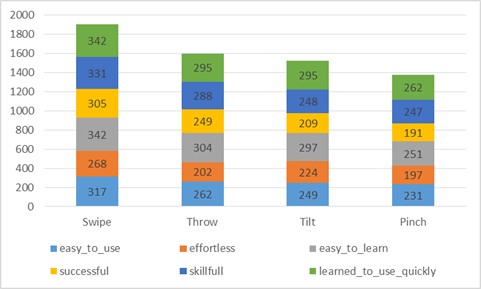
\includegraphics[width = 1\columnwidth , height = 6cm ]{images/survey-data.png}} 
	\caption{
		Cumulative values of survey questions per technique
	}
	\label{fig:surveyResult}
\end{figure}

One way MANOVA was applied after which ($F(18, 574.66)=5.118$ ,$p<0.000$; $Wilk's \lambda =0.657$,$partial  \eta\textsuperscript{2} = 0.131$ ) we can reject H\textsubscript{0} hypothesis, there was a statistically significant difference between scores in regards to technique. 
The post hoc revealed that in regards to: (1) It is easy to use there is no statistical difference between \throw, \tilt, and \pinch; (2) Using it is effortless there is no statistical difference between \throw, \tilt, and \pinch; (3) It is easy to learn to use there is no statistical difference between \tilt, and \throw; (4) I can use it successfully every time there is no statistical difference between \tilt, and \pinch; (5) I quickly became skillful with it there is no statistical difference between \pinch, and \tilt; (6) I learned how to use it quickly  there is no statistical difference between \throw, \tilt, and \pinch.